\documentclass[../main.tex]{subfiles}

\begin{document}

\problem{2}

\textit{Note: All calculations performed in Python using custom module designed to analyze isentropic flow and normal shocks. See appendix \ref{Problem2Python} and https://github.com/ejburke73/py-compressible-flow.}

\problempart{a} Plot the Mach number of the F-16 during its 20-minute flight.

\givens{}

Time series for \(p_t\) and \(p\), the total and static pressure, respectively, measured by the F-16's pitot-probe.
The flight data given covers a simple trajectory including a take-off, acceleration to max-speed, and deceleration to landing.

\assumptions{}

Let region 1 be the area upstream of the bow shock.
Let region 2 be the area \textit{immediately behind the shock} but not at the probe's stagnation point.
The static pressure measurement taken by the probe is valid for the static pressure \textit{upstream} of the shock.
The flow before and after the bow shock is isentropic, calorically perfect air. \(\gamma_{air} = 1.4, R_{air} = 287 \, \unit{\joule/\kilogram\cdot\kelvin}\).
The shock can be evaluated as a normal shock in front of the pitot probe.
A shock is only present in front of the pitot probe when the F-16 is traveling supersonically, \(M > 1\).
All flow is isentropically brought to rest at the tip of the pitot-probe.

\solution{}

During the subsonic portion of flight, the F-16's Mach number is found using isentropic equations relating \(p_t,\, p, \,\textrm{and} \, M\).

\[
    \frac{p_{t,1}}{p_1} = {\left({1 + \frac{\gamma-1}{2}M_1^2}\right)}^{\frac{\gamma}{\gamma-1}}
\]

Rearranging to isolate \(M\):

\[
    M_1 = \sqrt{
        \left[{{\left({\frac{p_{t,1}}{p_1}}\right)}^{\frac{\gamma-1}{\gamma}} - 1}\right]
        \frac{2}{\gamma-1}
    }
\]

During the subsonic portion of flight, we have data for the quantities \(p_{t,1} \, \textrm{and} \, p_1 \), and can easily solve for \(M_1\).
However, once the F-16 reaches supersonic velocities, this relation is no longer valid for our measurements. 
The total pressure measurement becomes the total pressure experienced by the probe \textit{behind the shock}, \(p_{t,2}\).
We must now find a new relationship using \(p_{t,2} \, , \, p_1 , \, \textrm{and} \, M_2\).
The ratio of total pressure behind a shock to static pressure in front of a shock can be expressed via the multiplication of other ratios we have isentropic/normal shock relations for.

\[
    \frac{p_{t,2}}{p_1} = 
    \frac{p_{t,2}}{p_2}
    \frac{p_2}{p_1}
\]

The isentropic relationship for total and static pressure has already been shown for the subsonic Mach caculations.

\[
    \frac{p_{t,2}}{p_2} = 
    {\left({1 + \frac{\gamma-1}{2}M_2^2}\right)}
    ^{\frac{\gamma}{\gamma-1}}
\]

The relationship connecting static pressure across a normal shock is given below:

\[
    \frac{p_2}{p_1} = 
    \left({
    \frac{2 \gamma}{\gamma+1} M_1^2 -
    \frac{\gamma-1}{\gamma+1}
    }\right)
\]

Combining these two equations yields an expression for \(p_{t,2}/p_1\) in terms of \(\gamma\), \(M_1\), and \(M_2\).

\[
    \frac{p_{t,2}}{p_1} = 
    {\left({1 + \frac{\gamma-1}{2}M_2^2}\right)}
    ^{\frac{\gamma}{\gamma-1}}
    \left({
    \frac{2 \gamma}{\gamma+1} M_1^2 -
    \frac{\gamma-1}{\gamma+1}
    }\right)
\]

We do not know \(M_1\) or \(M_2\), but we do have a normal shock relationship relating the two of them:

\[
    M_2^2
    =
    \frac{M_1^2 + \frac{2}{\gamma-1}}{\frac{2\gamma}{\gamma-1}M_1^2-1}
\]

Substituting this relation into our previous defined ratio:

\[
    \frac{p_{t,2}}{p_1} = 
    {\left({1 + \frac{\gamma-1}{2} {\left[{\frac{M_1^2 + \frac{2}{\gamma-1}}{\frac{2\gamma}{\gamma-1}M_1^2-1}}\right]} }\right)}
    ^{\frac{\gamma}{\gamma-1}}
    \left({
    \frac{2 \gamma}{\gamma+1} M_1^2 -
    \frac{\gamma-1}{\gamma+1}
    }\right)
\]

This equation cannot be solved by hand, so a numerical solver will be used in Python to determine the Mach number based on \(p_{t,2}/p_1\) while the F-16 is supersonic.
The final question that must be examined before calculating the F-16's Mach number during its flight is how to decide whether the F-16 is subsonic or supersonic without knowing the Mach number.
The answer comes by examining the limiting case of exactly sonic velocity, i.e. \(M=1\).
The isentropic total-to-static pressure ratio for \(M=1\) is given below, where \(p^*\) represents static pressure at sonic conditions.

\[
    \frac{p_{t}}{p^*} = 
    {\left({1 + \frac{\gamma-1}{2}}\right)}
    ^{\frac{\gamma}{\gamma-1}}
\]

Inserting our known value of \(\gamma\) yields the critical pressure ratio for sonic flight:

\[
    \frac{p_{t}}{p^*} \approx 1.89
\]

From this value we can determine when the F-16 reaches sonic velocities.
By definition, a normal shock at sonic conditions is an infinitely weak shock and is isentropic.
Examining the relationship for \(p_{t,2}/p^*\) at sonic conditions:

\[
    \frac{p_{t,2}}{p_1} = 
    {\left({1 + \frac{\gamma-1}{2} {\left[{\frac{1 + \frac{2}{\gamma-1}}{\frac{2\gamma}{\gamma-1}-1}}\right]} }\right)}
    ^{\frac{\gamma}{\gamma-1}}
    \left({
    \frac{2 \gamma}{\gamma+1}  -
    \frac{\gamma-1}{\gamma+1}
    }\right)
\]

\[
    \frac{p_{t,2}}{p_1} = 
    {\left({1 + \frac{\gamma-1}{2} \cancelto{1}{\left[{\frac{\gamma  + 1}{\gamma  + 1}}\right]} }\right)}
    ^{\frac{\gamma}{\gamma-1}}
    \left({
    \cancelto{1}{\frac{\gamma+1}{\gamma+1}}
    }\right)
\]

\[
    \frac{p_{t,2}}{p_1} = 
    {\left({1 + \frac{\gamma-1}{2}}\right)}
    ^{\frac{\gamma}{\gamma-1}}
\]

\[
    \frac{p_{t,2}}{p_1} \approx 1.89
\]

We have now proven that both the subsonic and supersonic relationships we have found converge onto the same value at the sonic condition.
Any time the pressure ratio from the pitot-probe exceeds this critical value, the F-16 is supersonic, and any time it is below, it is subsonic.

\discussion{}

Figure \ref{P_ratio} shows the time history of the pitot-probe's total to static pressure ratio, highlighting the critical threshold beyond which flight is supersonic.

\begin{figure}[h]
    \centering
    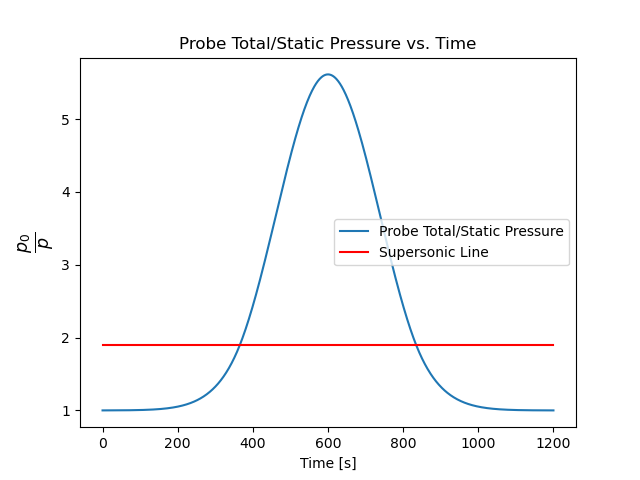
\includegraphics[scale=.7]{../images/problem_2/Probe_P_ratio_vs_Time_F16.png}
    \caption{Probe total-to-static pressure ratio and supersonic threshold}
    \label{P_ratio}
\end{figure}

Figure~\ref{MvsT_correct} shows the F-16's Mach number (Mach in region 1) over the time of its flight using the relationships we have defined.

\begin{figure}[h]
    \centering
    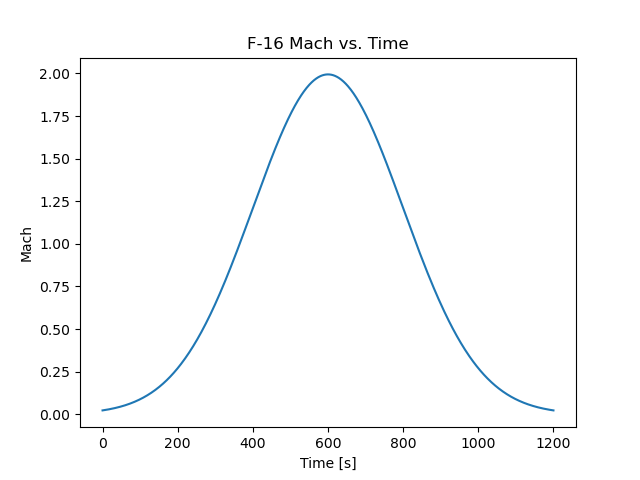
\includegraphics[scale=.7]{../images/problem_2/Mach_vs_Time_F16.png}
    \caption{F-16 Mach vs. Time during flight, calculated using isentropic and normal shock relations}
    \label{MvsT_correct}
\end{figure}

Figure \ref{MvsT_shockfree} shows a comparison of the F-16's Mach number calculated correctly, taking shocks into account, and calculated as if there were no shocks in front of the probe.

\begin{figure}[h]
    \centering
    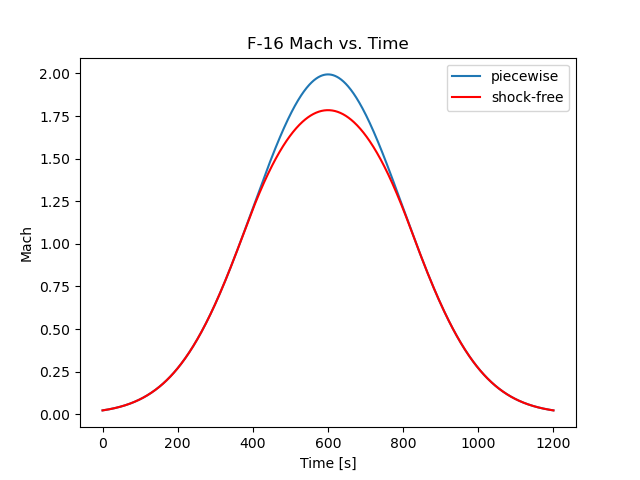
\includegraphics[scale=.7]{../images/problem_2/Mach_vs_Time_F16_Piecewise_Simple.png}
    \caption{F-16 Mach vs. Time during flight, calculated correctly and as if there were no shocks}
    \label{MvsT_shockfree}
\end{figure}

Figure \ref{MvsT_probe} shows the Mach number in region 2, which is immediately after the normal shock during supersonic flight.

\begin{figure}[h]
    \centering
    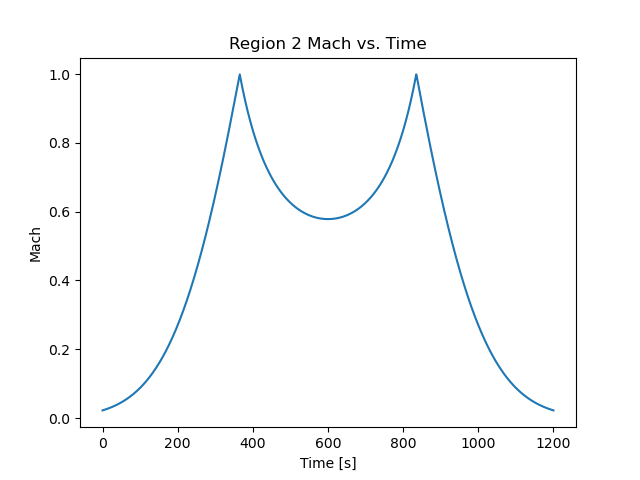
\includegraphics[scale=.7]{../images/problem_2/Mach_vs_Time_F16_Probe.png}
    \caption{Mach in region 2, upstream of pitot probe vs. Time during flight}
    \label{MvsT_probe}
\end{figure}

Figure \ref{MvsT_probe_aircraft} shows a comparison of the F-16's flight Mach number in region 1 and that of the post-shock flow in region 2.
Note that the region just upstream of the pitot probe experiences a local minimum Mach number when the F-16 is flying at its largest Mach number.
This is indicative of the fact that shock strength increases with incoming Mach number.

\begin{figure}[h]
    \centering
    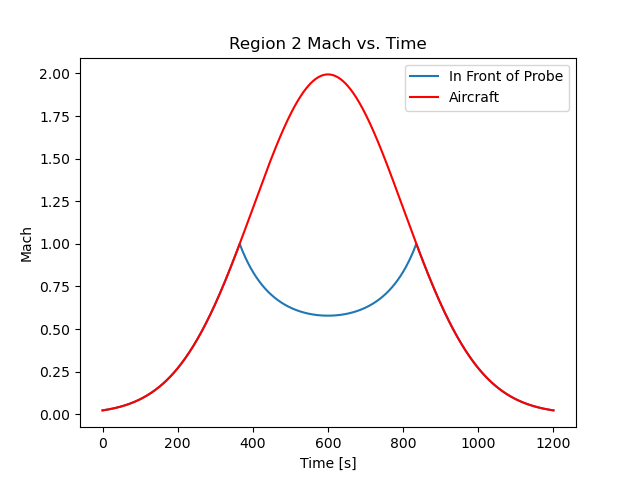
\includegraphics[scale=.7]{../images/problem_2/Mach_vs_Time_F16_Probe_Aircraft.png}
    \caption{Mach vs Time of flow in regions 1 (pre-shock/vehicle Mach) and 2 (post shock/before pitot) vs. Time during flight}
    \label{MvsT_probe_aircraft}
\end{figure}

\clearpage

\problempart{b} Plot the air temperature experienced at the tip of the probe for this 20-minute flight.

\givens{}

Time series for \(p_t\) and \(p\), the total and static pressure, respectively, measured by the F-16's pitot-probe.
The flight data given covers a simple trajectory including a take-off, acceleration to max-speed, and deceleration to landing.
There is a constant atmospheric temperature of \(T=298\,K\) at all altitudes in the trajectory.

\assumptions{}

Let region 1 be the area upstream of the bow shock.
Let region 2 be the area \textit{immediately behind the shock} but not at the probe's stagnation point.
The static pressure measurement taken by the probe is valid for the static pressure \textit{upstream} of the shock.
The flow before and after the bow shock is isentropic, calorically perfect air. \(\gamma_{air} = 1.4, R_{air} = 287 \, \unit{\joule/\kilogram\cdot\kelvin}\).
The shock can be evaluated as a normal shock in front of the pitot probe.
A shock is only present in front of the pitot probe when the F-16 is traveling supersonically, \(M > 1\).
All flow is isentropically brought to rest at the tip of the pitot-probe. Total temperature is constant across a shock because shocks are adiabatic.

\solution{}

Given a constant freestream air temperature of \(T_\infty = 298 K\) and the previously calculated vehicle Mach number, we can determine the total temperature experienced by the F-16 over the duration of its flight using the following isentropic relationship:

\[
    \frac{T_{t,1}}{T_1} = 1 + \frac{\gamma-1}{2} M_1^2
\]

\[
   T_{t,1} = 298 \, [K]* \left({1 + \frac{\gamma-1}{2} M_1^2}\right)
\]

We know that shocks are adiabatic and therefore total temperature across a shock is constant.

\[
    T_{t,1} = T_{t,2}
\]

Because we are assuming that the tip of the probe is a stagnation point \((M=0)\), total temperature is equal to static temperature for the probe.

\[
    T_{t,2} = T_{t,probe} = T_{probe}
\]

Figure \ref{Probe_temp} shows the time history of temperature experienced at the tip of the pitot probe.

\begin{figure}[h]
    \centering
    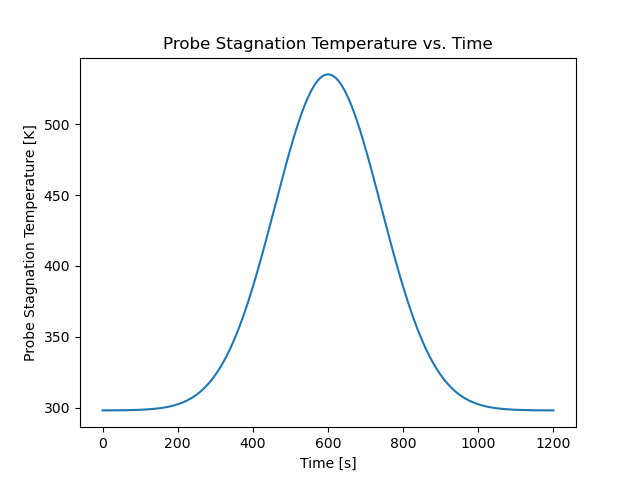
\includegraphics[scale=.7]{../images/problem_2/Probe_T_t_vs_Time_F16.png}
    \caption{Pitot Probe Total Temperature vs. Time}
    \label{Probe_temp}
\end{figure}

These temperatures are safely below the melting point of aluminum.

\end{document}